La instalación de los programas necesarios para el desarrollo de este Trabajo de Fin de Grado se ha realizado en un equipo con Ubuntu 22.04 LTS. Las características hardware del equipo son las siguientes:

\begin{multicols}{2}
\begin{itemize}
    \item Procesador: AMD Ryzen 5 2600 Six-Core @ 12x 3,4GHz
    \item Tarjeta gráfica: NVIDIA GeForce RTX 2060
    \item Memoria RAM: 16 GB
    \item 256 GB SSD
    \item Sistema operativo: Ubuntu 22.04 LTS
\end{itemize}
\end{multicols}

\section{Instalación y configuración de GNS3}
\label{Apendice1:instalacion_gns3}
\noindent
Para instalar GNS3 se va a utilizar el gestor de paquetes de Ubuntu, \texttt{apt}.

\begin{lstlisting}[language=bash]
sudo add-apt-repository ppa:gns3/ppa
sudo apt update
sudo apt install gns3-gui gns3-server
\end{lstlisting}

\noindent
Una vez instalado GNS3 se comprobará que se ha instalado correctamente ejecutando el siguiente comando:

\begin{lstlisting}[language=bash]
gns3 --version
\end{lstlisting}

\noindent
y así se comprobará que se ha instalado correctamente. En este caso, la versión que se ha usado es la 2.2.54. Por otro lado, GNS3 permite la integración de imágenes QEMU/KVM para emular dispositivos de red. Para ello, es recomendable 
contar con soporte para \textbf{KVM} habilitado en el sistema. Esto mejora el rendimiento de las máquinas 
virtuales dentro de GNS3. Para hacer esta comprobación se va a utilizar el paquete \texttt{cpu-checker}. La 
instalación del mismo se hace con:

\begin{lstlisting}[language=bash]
sudo apt install cpu-checker
\end{lstlisting}

\noindent
Una vez instalado el paquete, se puede comprobar si el sistema tiene soporte para KVM ejecutando \lstinline|kvm-ok|:

\begin{lstlisting}[language=bash]
INFO: /dev/kvm exists
KVM acceleration can be used
\end{lstlisting}

\noindent
El resultado debería ser el que se muestra en pantalla. Si no es así, se debe habilitar la virtualización por hardware o que esté desactivada en label BIOS. 

\vspace{1em}
\noindent
Para que todo funcione correctamente, se debe modificar los permisos del ejecutable \texttt{ubridge} para 
que pueda ser ejecutado por el usuario que ejecuta GNS3.

\begin{lstlisting}[language=bash]
sudo chmod 755 /usr/bin/ubridge
\end{lstlisting}

\noindent
Además, para poder hacer uso de las máquinas virtuales dentro del simulador hay que hacer funcionar KVM. La instalación de este componente se debió hacer al instalar GNS3.
Sin embargo, para tener los permisos necesarios debemos añadir el usuario que ejecuta GNS3 al grupo \texttt{kvm}.

\begin{lstlisting}[language=bash]
sudo adduser $USER kvm
\end{lstlisting}

\noindent
Una vez hecho esto, se debe reiniciar el sistema para que los cambios surtan efecto. Una vez reiniciado el sistema, se puede iniciar GNS3 y comprobar que todo funciona correctamente.

\section{Instalación de VirtualBox}
\label{Apendice1:instalacion_virtualbox}
Para instalar VirtualBox \cite{virtualbox} se debe descargar el paquete de instalación desde la página oficial de VirtualBox para la versión del sistema operativo que se esté usando. En este caso, se está usando Ubuntu 22.04 LTS, por lo que se debe descargar el paquete de instalación para esta versión.

\begin{figure}[H]
	\centering
	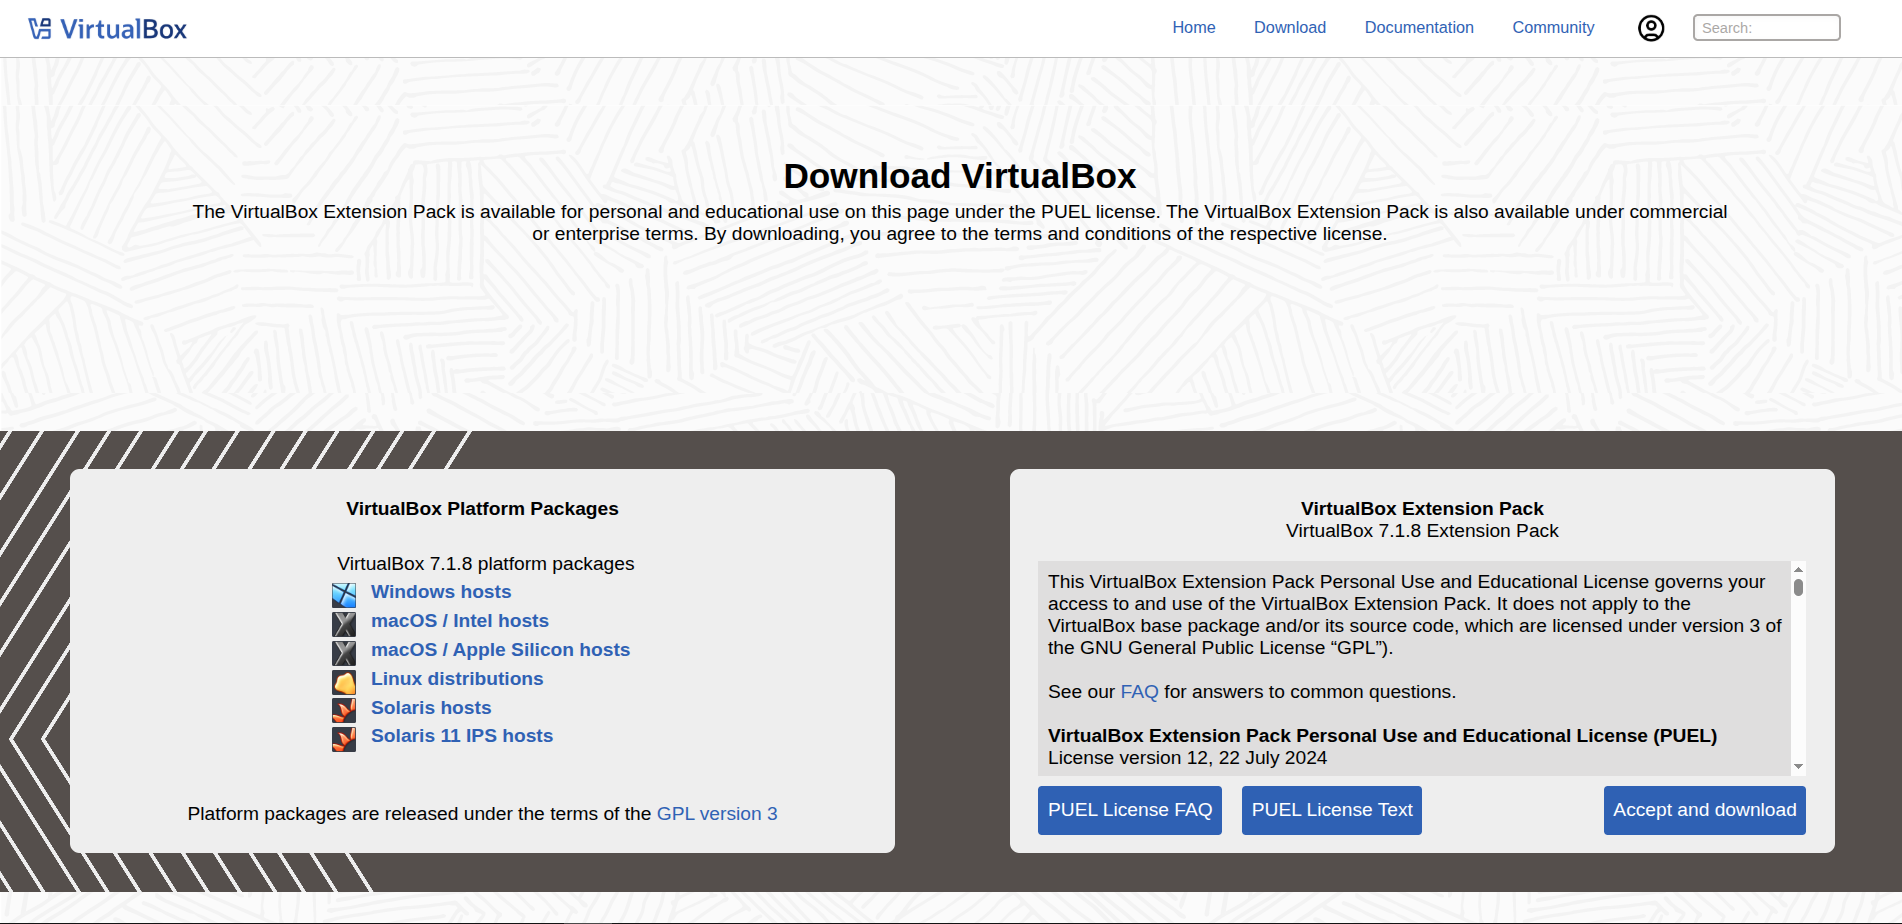
\includegraphics[width=1\textwidth]{images/virtualbox_download.png}
	\caption{Descarga de VirtualBox}
	\label{fig:virtualbox_download}
\end{figure}

\noindent
Elegimos la opción de \texttt{Download VirtualBox for Linux hosts}, en este caso, y elegimos la distribución de Linux que se esté usando. En este caso, se está usando Ubuntu 22.04 LTS, por lo que se debe elegir la opción de \texttt{Ubuntu 22.04 (64-bit)}.

\begin{figure}[H]
	\centering
	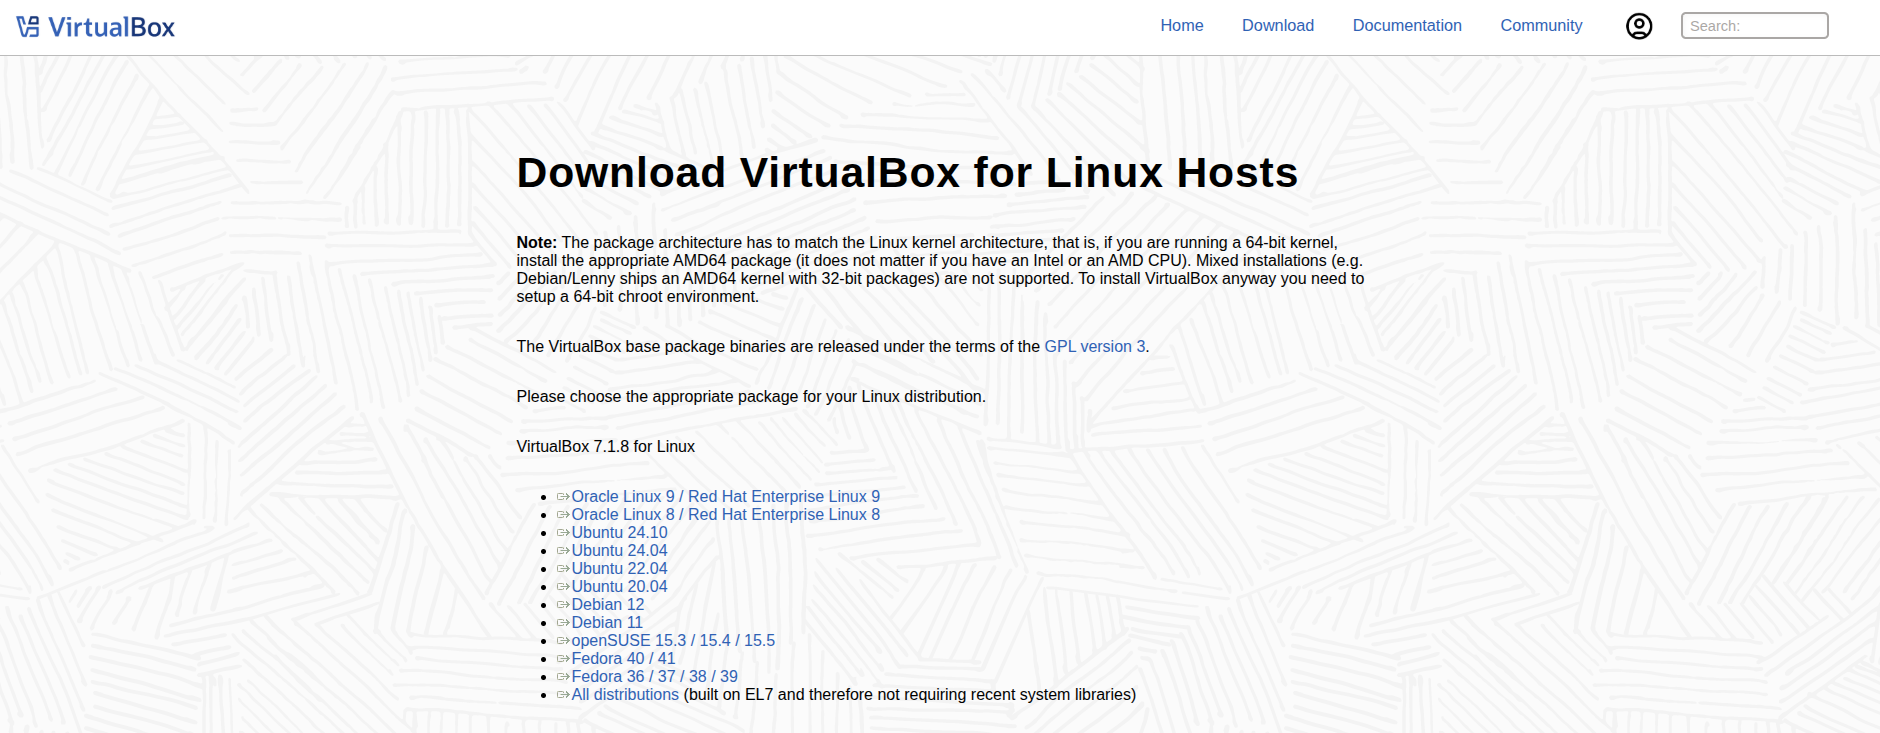
\includegraphics[width=0.9\textwidth]{images/virtualbox_download_2.png}
	\caption{Descarga de VirtualBox}
	\label{fig:virtualbox_download_2}
\end{figure}

\noindent
Una vez descargado el paquete, se debe instalar. Para ello, se debe abrir una terminal y navegar hasta la carpeta donde se ha descargado el paquete.
\begin{lstlisting}[language=bash]
cd ~/Descargas
sudo dpkg -i virtualbox-7.1_7.1.8-168469~Ubuntu~jammy_amd64.deb
\end{lstlisting}

\noindent
Si se produce algún error de dependencias, se puede solucionar ejecutando el siguiente comando:
\begin{lstlisting}[language=bash]
sudo apt --fix-broken install
\end{lstlisting}

\noindent
Una vez instalado VirtualBox, se puede comprobar que se ha instalado correctamente ejecutando el siguiente comando:
\begin{lstlisting}[language=bash]
virtualbox --help
\end{lstlisting}

\noindent
y así se comprobará que se ha instalado correctamente. En este caso, la versión que se ha usado es la 7.1.8.

\subsection{Instalación FreePBX}
\label{Apendice1:instalacion_freepbx}
Para instalar FreePBX \cite{freepbx}, primero es necesario acceder a la página oficial y descargar el instalador correspondiente a la versión del sistema operativo que se esté utilizando. En la sección \texttt{Download}, se debe desplegar la opción \texttt{View Previous Versions} para seleccionar la versión deseada. En este caso, se ha descargado la imagen ISO de la versión \texttt{SNG7-PBX16-64bit-2302-1}, como se muestra en la figura~\ref{fig:freepbx_download}.
\begin{figure}[H]
	\centering
	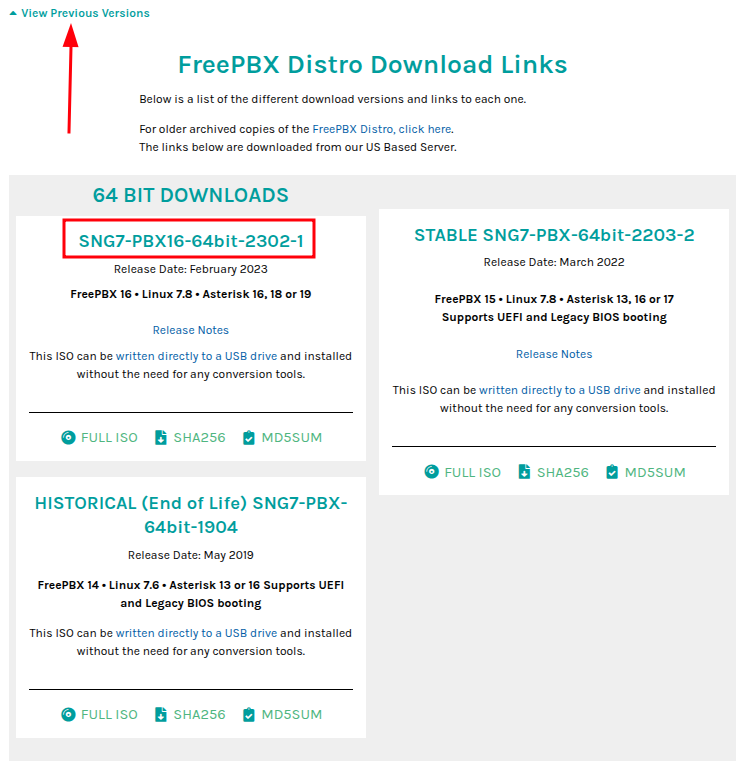
\includegraphics[width=0.7\textwidth]{images/freepbx_download.png}
	\caption{Descarga de FreePBX}
	\label{fig:freepbx_download}
\end{figure}

\vspace{1em}
\noindent
Una vez descargado el paquete, se debe montar la imagen ISO en una máquina virtual de VirtualBox.
Para ello, se debe crear una nueva máquina virtual en VirtualBox, seleccionamos \texttt{Nueva} 
y seleccionar la imagen ISO descargada como disco de arranque y se configura la máquina virtual con los siguientes parámetros:
\begin{multicols}{2}
\begin{itemize}
    \item Nombre: FreePBX
    \item Tipo: Linux
    \item Versión: Red Hat (64-bit)
		\item Omitir instalación desatendida: No
    \item Memoria RAM: 1024 MB
    \item Procesador: 1 CPU
		\item Disco duro virtual: 20 GB 
\end{itemize}
\end{multicols}

\begin{figure}[H]
    \centering
    \begin{minipage}{0.49\textwidth}
        \centering
        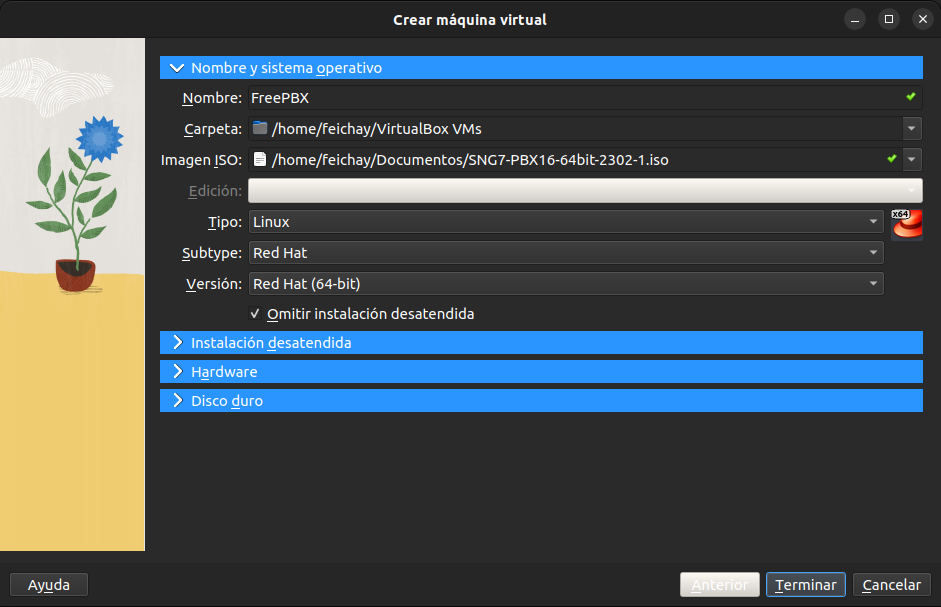
\includegraphics[width=\textwidth]{images/freepbx_virtualbox.png}
    \end{minipage}\hfill
    \begin{minipage}{0.49\textwidth}
        \centering
        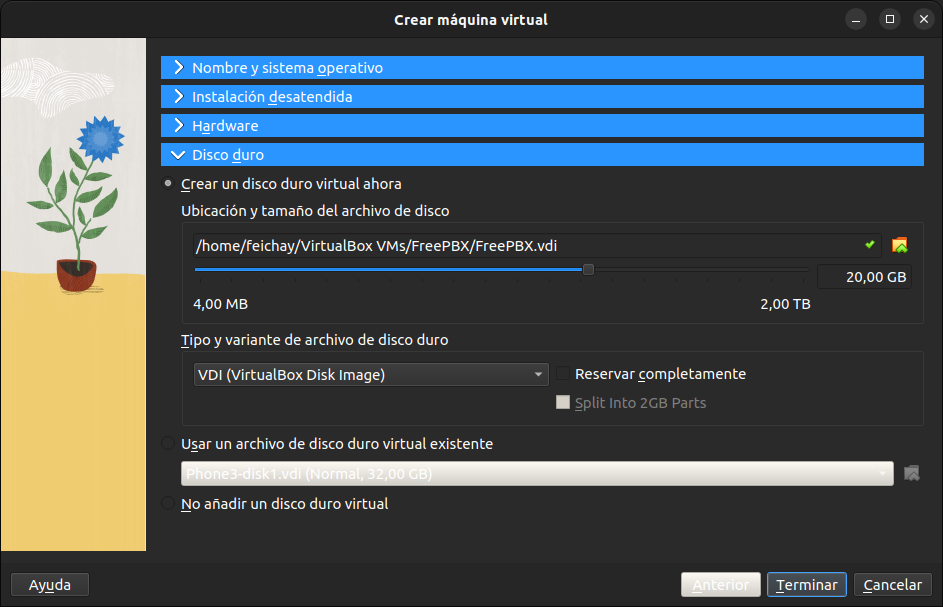
\includegraphics[width=\textwidth]{images/freepbx_virtualbox_2.png}
    \end{minipage}
		\caption{Configuración de la máquina virtual para FreePBX}
		\label{fig:freepbx_virtualbox}
\end{figure}

Una vez creada la máquina virtual, se debe configurara dos adaptadores de red. Pero antes, se debe crear un nuevo \texttt{Adaptador solo anfitrión} en VirtualBox, 
para ello ejecutamos el siguiente comando en la terminal:
\begin{lstlisting}[language=bash]
sudo VBoxManage hostonly create
\end{lstlisting}

\noindent
Esto creará un nuevo adaptador de red solo para el anfitrión. A continuación, se debe configurar los adaptadores de red para la máquina virtual FreePBX. Para ello, se debe seleccionar la máquina virtual creada y hacer clic en \texttt{Configuración}. En la sección \texttt{Red}, se debe seleccionar el adaptador \texttt{Adaptador 1} y configurarlo de la siguiente manera:
\begin{multicols}{2}
\begin{itemize}
		\item Habilitar adaptador de red: Sí
		\item Conectado a: Adaptador puente
		\item Nombre: <nombre de la interfaz de red del equipo>
		\item Promiscuo: Permitir todo
\end{itemize}

\columnbreak

\begin{itemize}
		\item Tipo de adaptador: Intel PRO/1000 MT Desktop (82540EM)
		\item Dirección MAC: Dejar en blanco
		\item Cable conectado: Sí
\end{itemize}
\end{multicols}

\noindent
A continuación, se debe configurar el \texttt{Adaptador 2} de la siguiente manera:
\begin{multicols}{2}
\begin{itemize}
		\item Habilitar adaptador de red: Sí
		\item Conectado a: Adaptador solo anfitrión
		\item Nombre: vboxnet0
		\item Promiscuo: Permitir todo
\end{itemize}

\columnbreak

\begin{itemize}
		\item Tipo de adaptador: Intel PRO/1000 MT Desktop (82540EM)
		\item Dirección MAC: Dejar en blanco
		\item Cable conectado: Sí
\end{itemize}
\end{multicols}

\noindent
Una vez creada los adaptadores de red, vamos a asignar una dirección IP al adaptador \texttt{Adaptador sólo anfitrión} creado anteriormente. Esto es para usar esta interfaz en la simulación de GNS3.
Para ello, en la parte superior izquierda de la ventana de VirtualBox, donde aparece \texttt{Herramientas} le damos al boton de propiedades y seleccionamos la pestaña \texttt{Red}. Y una vez dentro de
la pestaña, vemos la el adaptador creado anteriormente, \texttt{vboxnet0}, y abajo de este configuramos la dirección IP y la máscara de subred. En este caso, se ha configurado la dirección IP 
\texttt{192.168.1.135} y la máscara de subred \texttt{255.255.255.240}.

\begin{figure}[H]
	\centering
	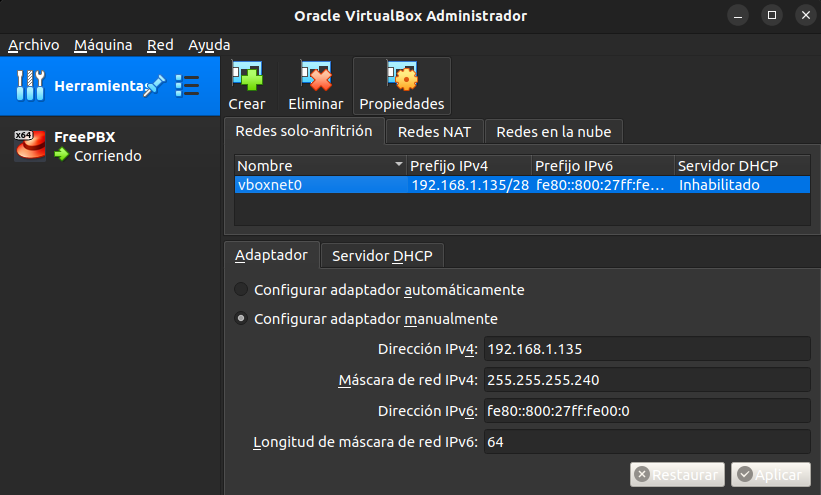
\includegraphics[width=0.8\textwidth]{images/freepbx_virtualbox_3.png}
	\caption{Configuración de la red en VirtualBox}
	\label{fig:freepbx_virtualbox_red}
\end{figure}

\noindent
Una vez configurada la red, se debe iniciar la máquina virtual y seguir las instrucciones de instalación de FreePBX. Selecionamos la primera opción y pulsamos \texttt{Enter} para iniciar la instalación. A continuación, saldrá \texttt{FreePBX Standard} y pulsamos \texttt{Enter} nuevamente para continuar con la instalación. Ya dentro de panel de configuración de FreePBX, hay que configurar el usuario y la contraseña para el usuario \texttt{root}. Para simplicidad, se ha configurado el usuario \texttt{root} con la contraseña \texttt{root}. Y esperamos a que se complete la instalación. Una vez completada la instalación, vamos a apagar la máquina virtual para eliminar el disco de instalación y arrancar desde el disco duro virtual.

\begin{figure}[H]
    \centering
    \begin{minipage}{0.49\textwidth}
        \centering
        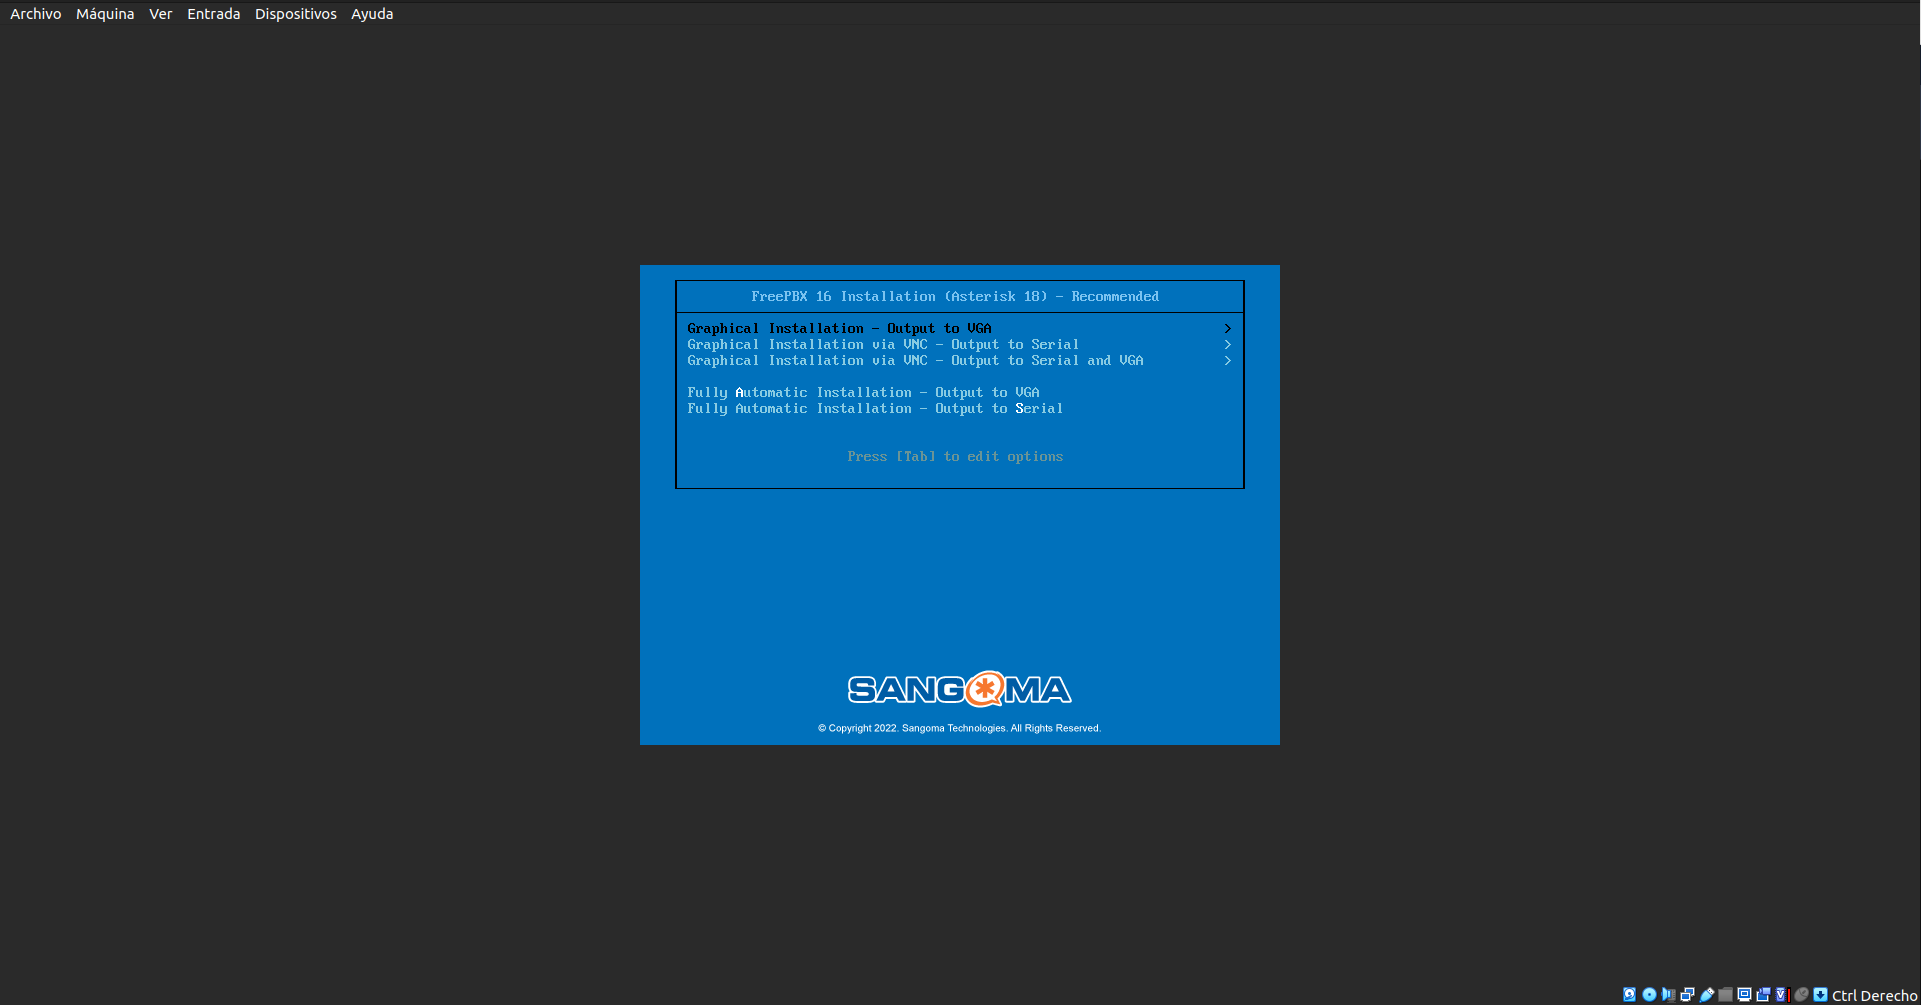
\includegraphics[width=\textwidth]{images/freepbx_installation_1.png}
    \end{minipage}\hfill
    \begin{minipage}{0.49\textwidth}
        \centering
        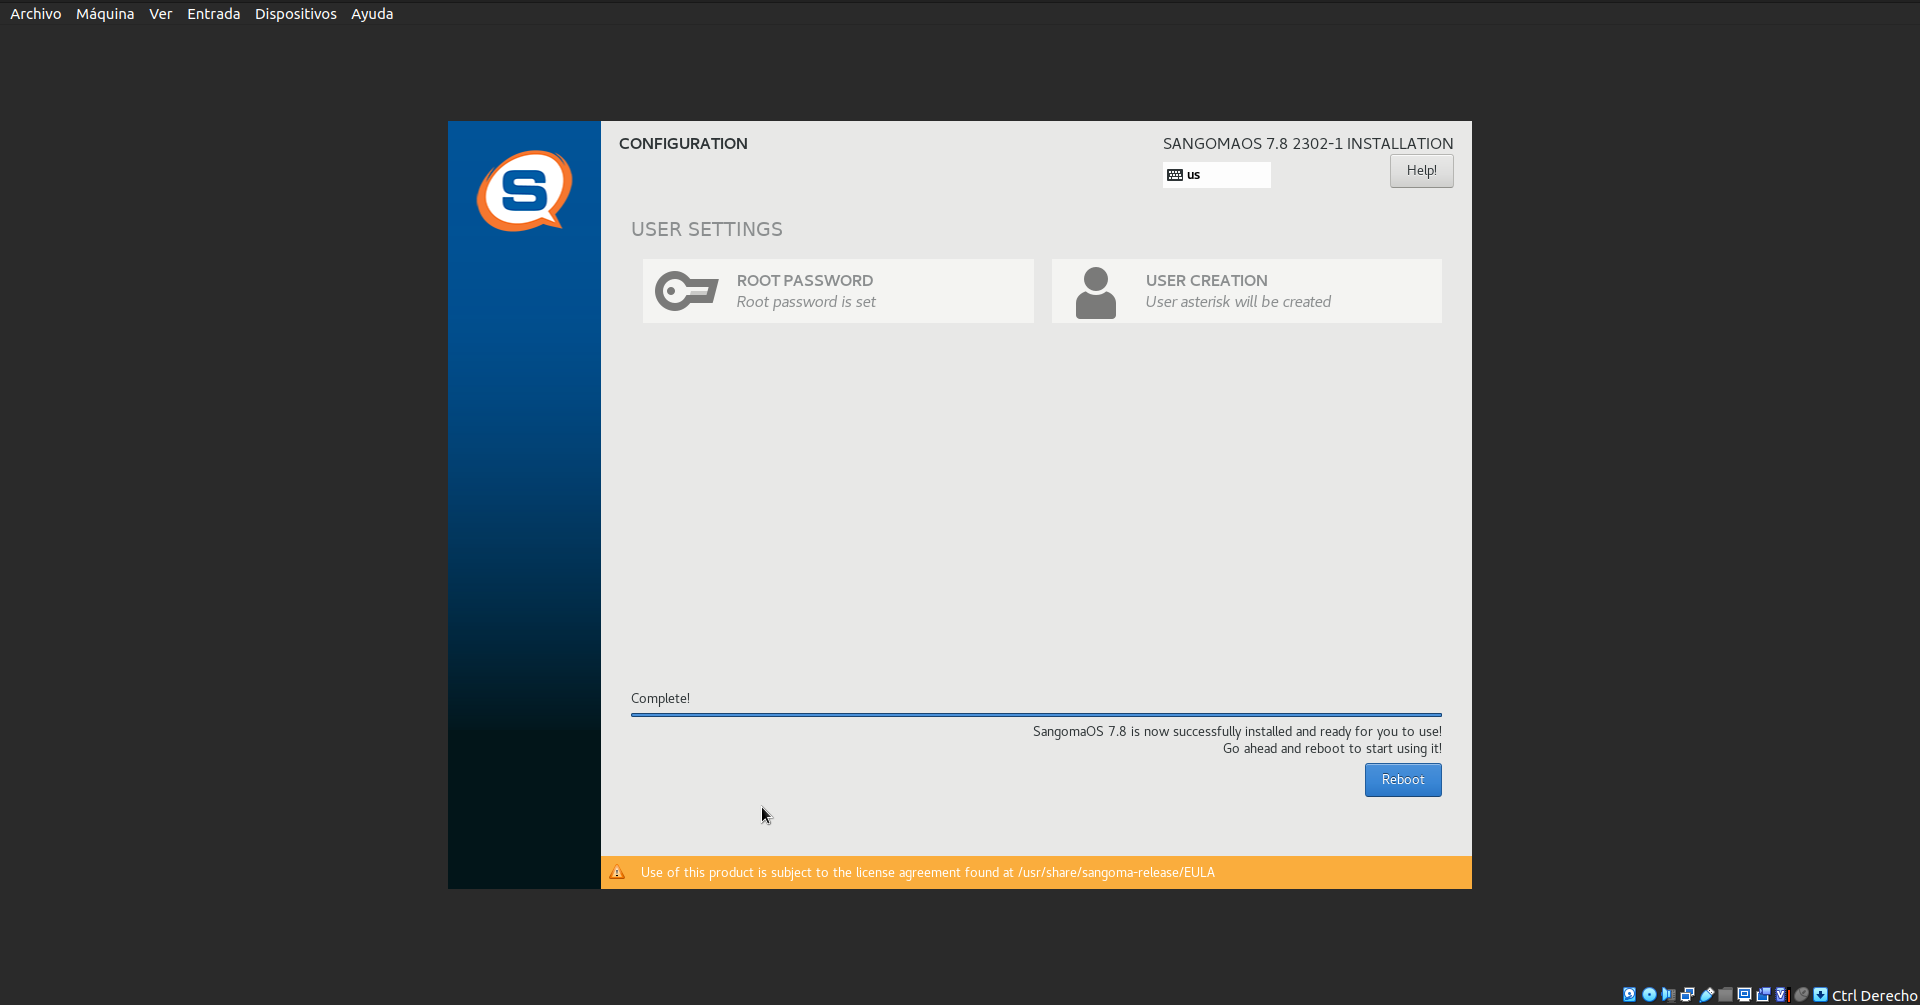
\includegraphics[width=\textwidth]{images/freepbx_installation_5.png}
    \end{minipage}
		\caption{Configuración de la máquina virtual para FreePBX}
		\label{fig:freepbx_installation_1}
\end{figure}

\noindent
Para ello, vamos a la configuración de la máquina virtual y en la sección \texttt{Almacenamiento} eliminamos el disco de instalación como se muestra en la figura~\ref{fig:freepbx_installation_6}.

\begin{figure}[H]
	\centering
	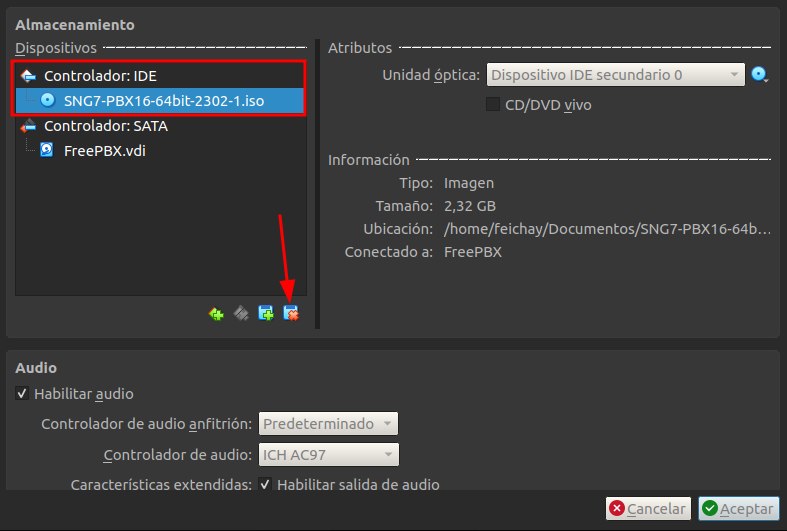
\includegraphics[width=0.8\textwidth]{images/freepbx_installation_6.png}
	\caption{Instalación de FreePBX}
	\label{fig:freepbx_installation_6}
\end{figure}

\noindent
Una vez eliminado el disco de instalación, iniciamos la máquina virtual y accedemos al panel de configuración de FreePBX con la dirección IP que se le ha asignado a la máquina virtual. En la figura~\ref{fig:freepbx_terminal.png} se muestra la dirección IP asignada a la máquina virtual, que en este caso es \texttt{192.168.1.31}.
\begin{figure}[H]
	\centering
	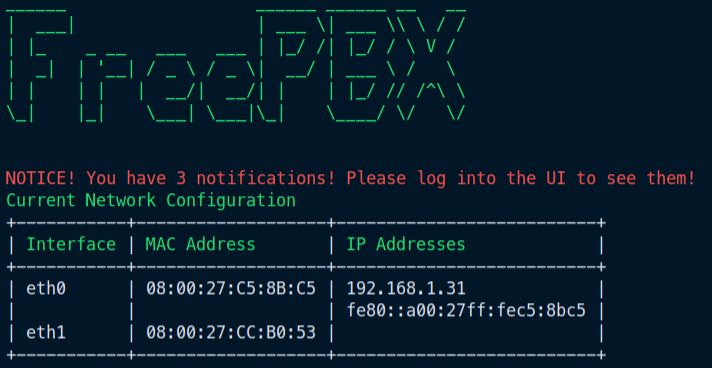
\includegraphics[width=0.8\textwidth]{images/freepbx_terminal.png}
	\caption{Panel de configuración de FreePBX}
	\label{fig:freepbx_terminal.png}
\end{figure}

\noindent
Para acceder al panel de configuración de FreePBX, se debe abrir un navegador web y acceder a la dirección IP asignada a la máquina virtual. En este caso, se ha accedido a la dirección 
\url{http://192.168.1.31/admin}. Una vez accedido al panel de configuración, se debe de crear el usuario administrador. Para simplificar, se ha creado el usuario \texttt{admin} con la contraseña \texttt{admin}.

\begin{figure}[H]
	\centering
	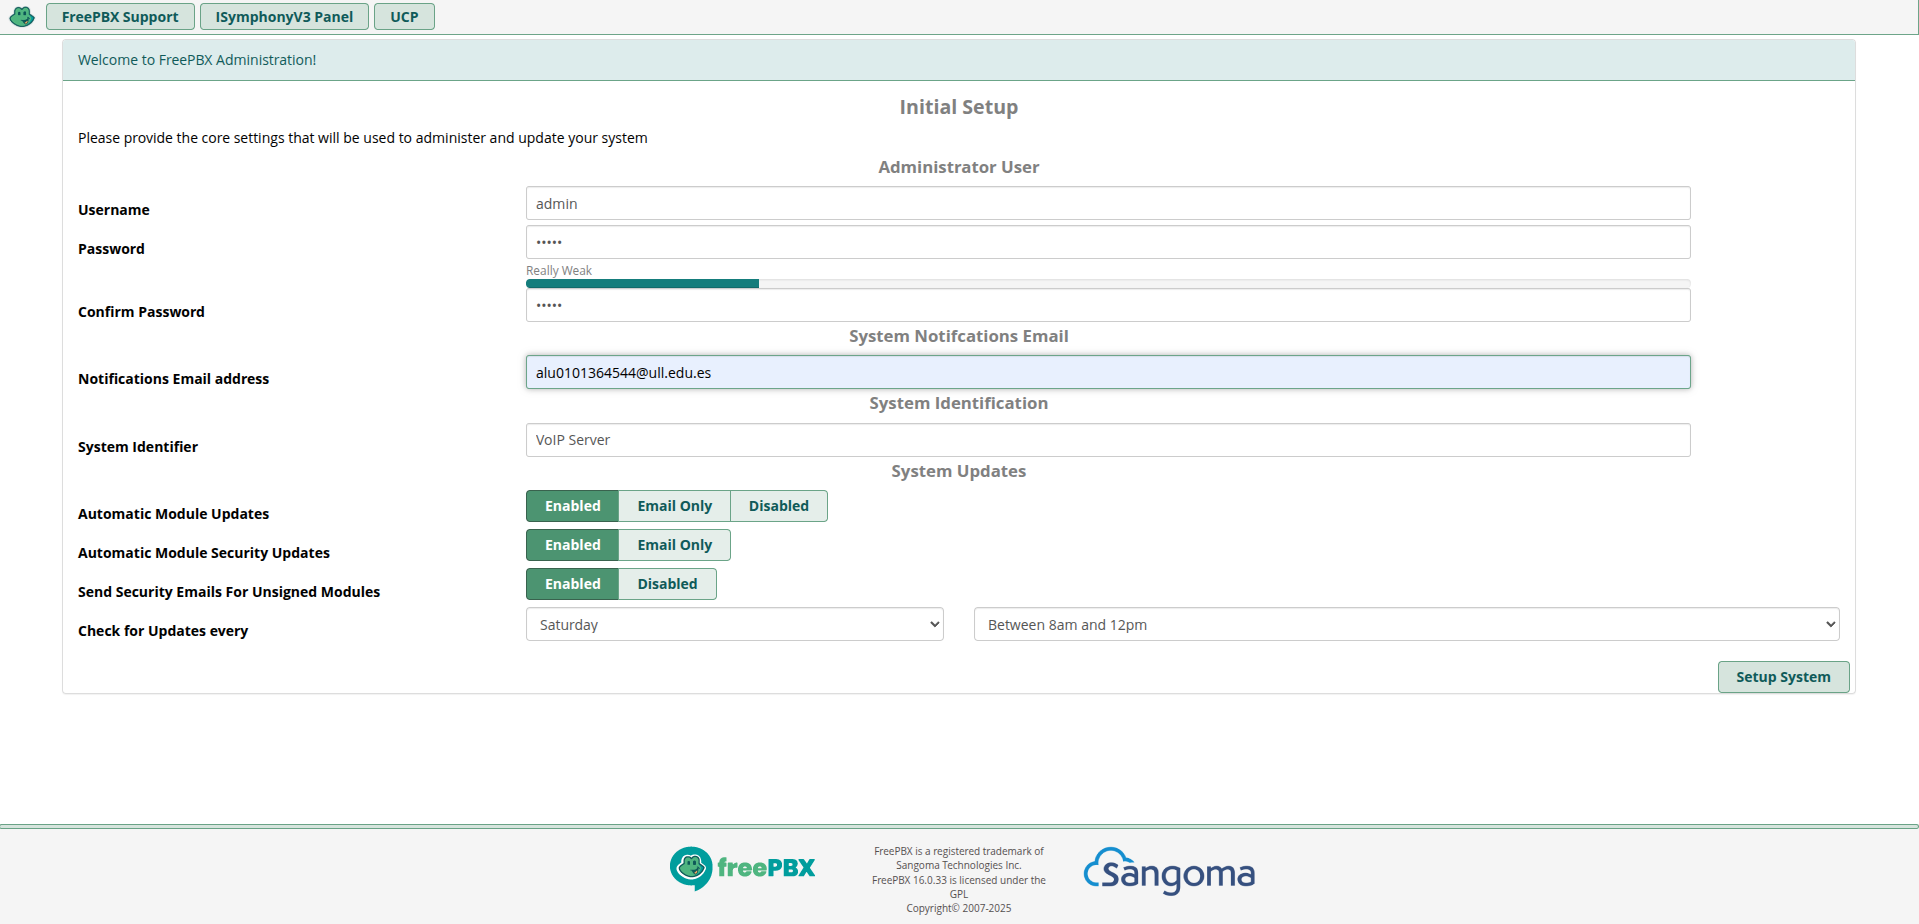
\includegraphics[width=0.8\textwidth]{images/freepbx_configuration_admin.png}
	\caption{Configuración de FreePBX}
	\label{fig:freepbx_configuration_admin}
\end{figure}

\subsection{Instalacion Softphone}
\label{Apendice1:instalacion_softphone}
Para la simulación de telefonos IPs en GNS3, se ha utilizado una máquina virtual ligera con el sistema operativo Windows 7 obtenido de un video tutorial de Youtube \cite{youtube_carlos_carrillo} de \texttt{Método para simular redes VoIP en GNS3}. Para instalar la máquina virtual, se ha descargado desde el enlace que proporciona el video tutorial y se ha importado a VirtualBox como un disco duro virtual en formato \texttt{.vdi} con el sistema operativo Windows 7 instalado y ya configurado.

\vspace{1em}
\noindent
Para importar la máquina virtual, se debe abrir VirtualBox y seleccionar \texttt{Nueva} para crear una nueva máquina virtual. Se debe poner un nombre, por ejemplo \texttt{Phone1}, seleccionar el tipo de sistema operativo, \texttt{Windows}, y la versión como \texttt{Windows 7 (64-bit)}. 

\begin{figure}[H]
	\centering
	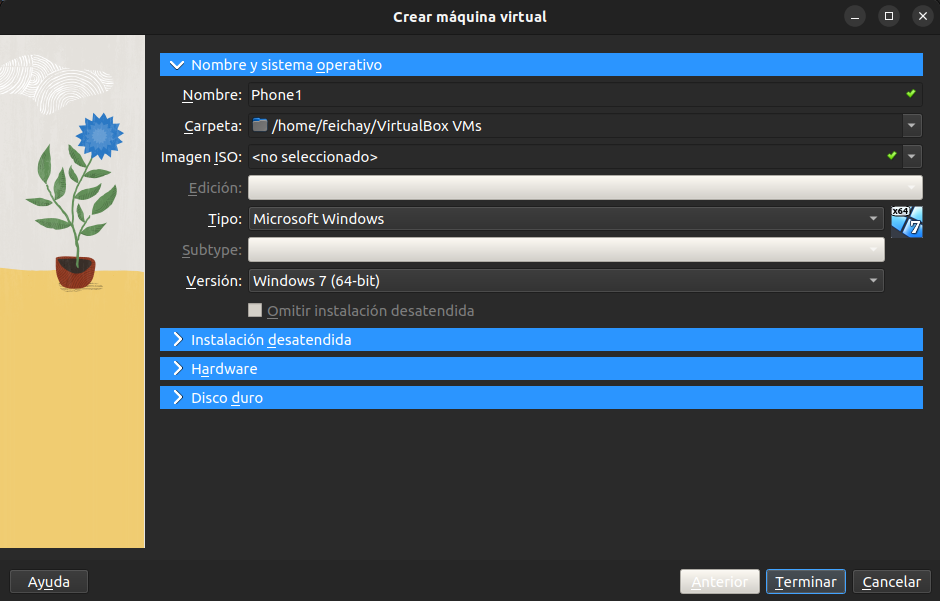
\includegraphics[width=0.8\textwidth]{images/softphone_1.png}
	\caption{Configuración de la máquina virtual para Softphone}
	\label{fig:softphone_1}
\end{figure}

\noindent
Luego, se debe asignar una cantidad de memoria RAM (256 MB es suficiente) y 1 CPU.

\begin{figure}[H]
	\centering
	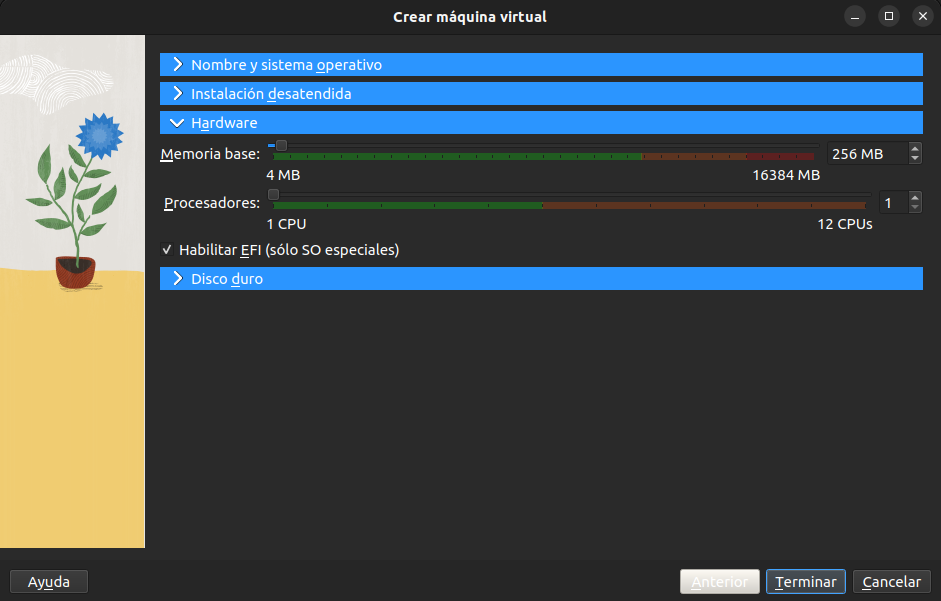
\includegraphics[width=0.8\textwidth]{images/softphone_2.png}
	\caption{Configuración de la máquina virtual para Softphone}
	\label{fig:softphone_2}
\end{figure}

\noindent
Por último, se debe seleccionar el disco duro virtual que se ha descargado previamente. Para ello, se debe seleccionar la opción \texttt{Usar un archivo de disco duro virtual existente} y seleccionar el archivo descargado.

\begin{figure}[H]
	\centering
	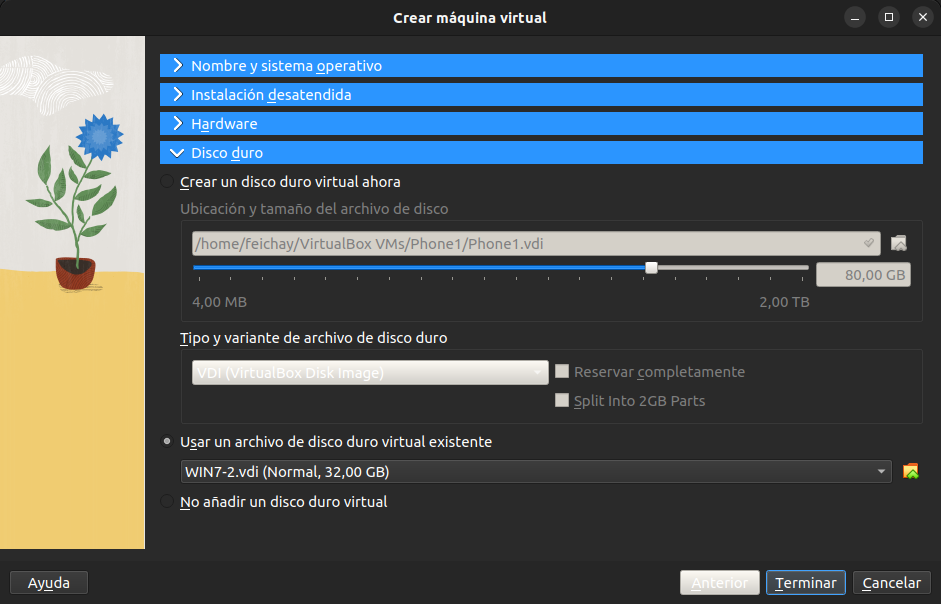
\includegraphics[width=0.8\textwidth]{images/softphone_3.png}
	\caption{Configuración de la máquina virtual para Softphone}
	\label{fig:softphone_3}
\end{figure}

\section{Instalación de Docker}
\label{Apendice1:instalacion_docker}
Para instalar Docker \cite{docker_ubuntu} y Docker Compose \cite{docker_compose_ubuntu} en Ubuntu, se deben seguir los siguientes pasos:

\subsection{Añadir el repositorio Docker}
Primero, instalar todas las dependencias necesarias usando el siguiente comando:
\begin{lstlisting}[language=bash]
sudo apt update
sudo apt install apt-transport-https ca-certificates curl software-properties-common -y
\end{lstlisting}

Después de instalar todas las dependencias, hay que descargar y añadir la clave GPG de Docker CE (Docker Community Edition) con el siguiente comando:
\begin{lstlisting}[language=bash]
curl -fsSL https://download.docker.com/linux/ubuntu/gpg | sudo apt-key add -
\end{lstlisting}

Ahora, añadimos el repositorio de Docker CE con el siguiente comando. Es importante notar que aunque la guía original mencione "focal" (para Ubuntu 20.04), para Ubuntu 22.04 (Jammy Jellyfish) se debería usar "jammy". Sin embargo, si se sigue una guía específica que indica "focal" y funciona, se puede mantener, pero es recomendable usar la versión correspondiente a la distribución:
\begin{lstlisting}[language=bash]
sudo add-apt-repository "deb [arch=amd64] https://download.docker.com/linux/ubuntu $(lsb_release -cs) stable"
\end{lstlisting}
O, si se desea usar "focal" explícitamente:
\begin{lstlisting}[language=bash]
sudo add-apt-repository "deb [arch=amd64] https://download.docker.com/linux/ubuntu focal stable"
\end{lstlisting}

Por último, verificar que se ha añadido el repositorio con el siguiente comando:
\begin{lstlisting}[language=bash]
apt-cache policy docker-ce
\end{lstlisting}

\subsection{Instalar Docker y Docker Compose}
Ahora, hay que instalar los paquetes de Docker usando el siguiente comando:
\begin{lstlisting}[language=bash]
sudo apt update
sudo apt install docker-ce -y
\end{lstlisting}

Una vez está Docker instalado, hay que verificar que Docker está corriendo correctamente:
\begin{lstlisting}[language=bash]
sudo systemctl status docker
\end{lstlisting}

Después, hay que instalar Docker Compose. La forma de instalar Docker Compose puede variar. Una forma común es descargarlo directamente desde GitHub. Sin embargo, si está disponible en los repositorios (como `docker-compose-plugin` o `docker-compose` v2), esa sería la forma preferida. La instrucción `apt install docker-compose -y` instalará la versión disponible en los repositorios de Ubuntu, que podría ser la v1. Para la v2, que se integra como un plugin de Docker CLI, los pasos serían diferentes.
\begin{lstlisting}[language=bash]
sudo apt install docker-compose -y
\end{lstlisting}
Para verificar la instalación de Docker Compose:
\begin{lstlisting}[language=bash]
docker-compose --version
\end{lstlisting}